\documentclass[12pt]{report}
\usepackage{mathptmx}
\usepackage[left=2.5cm, right=2.5cm, top=2.5cm, bottom=2.5cm]{geometry}
\usepackage[slovak]{babel}
\usepackage{pdfpages}
\linespread{1.0} 

\author{Mykyta Fedorin}
\title{BikeXpress}
\date{}

\begin{document}

\maketitle

\chapter{Použivateľská špecifikácia}
\section{Stručný úvod do problematiky}
\subsection{Vseobecny scenar pouzitia}

Firma BikeXpress sa zaoberá požičaním bicyklov a žiada o vytvorenie softvéru prevádzky(ďalej
len Systém). Distribúciu služieb bude robiť pomocou staníc z bicyklami, ktore umiestni po celej
Bratislave. Každá stanica bude obsahovať hlavný riadiaci prístroj. Tento prístroj bude riadiť za-
mok, pomocou ktorého je uzamknuty každý z bicyklov v danej stanici. Systém mal by umožniť
zákazníkom používať platené služby pozicania bicyklov firmy BikeXpress. Služby budú pozostávať
z plateného pozicania bicykla, s cieľom pomôcť zákazníkovi sa dostať tam, kde potrebuje a vrátiť
bicykel naspäť do bližšej stanice.

Systém je rozdelený na dve funkčné časti. Prvá časť je určená pre majiteľa (správcu) služby bike
sharing a druhá pre ľudí (zákazníkov), ktorí chcú využívať bicykle správcu na vlastnú prepravu po
meste. Správca ma úplnú kontrolu nad celým systémom, t.j. vidí všetky servisné dáta pre konkrétny
bicykel, vie nastavovať HW aj SW pre každý bicykel zvlášť alebo pre celú skupinu bicyklov a to všetko
vzdialene. 

Tak isto vidí aj štatistiku používania bicyklov. Systém ponúka správcovi definovať rôzne
tarify prispôsobené napr. podľa dátumu a času. V systéme je integrovaný aj mailový klient a SMS brána,
ktoré slúžia na komunikáciu so zákazníkmi a posielaní upozornení alebo informačných správ pre
zákazníkov. Zaujímavou funkciou je aj tzv. servisný modul, ktorý upozorňuje správcu o blížiacich sa
termínoch technickej údržby bicyklov. Napr. po prejdení určitých kilometrov sa musia skontrolovať
brzdy, prehadzovačka, dezén, svetlá. 

Pre zákazníkov je určená webová aplikácia a mobilná aplikácia
(Android, IOS). Ich funkcionalita obsahuje zobrazenie on-line mapy obsadenosti bicyklov a zobrazenie
mapy staníc bike sharing-u. Každý zákazník má svoj používateľský profil, kde vidí svoje štatistiky
a históriu vypožičaní a platieb. Tak isto sa zákazníkovi zobrazujú v profile aj rôzne akcie a zľavy,
ktorých odber si môže aktivovať alebo zablokovať. Aplikácia vie vykonať bezpečnú online platbu.
Mobilná aplikácia dokáže to isté ako webová, ale naviac má podporu pre rýchle vypožičanie pomocou
NFC/snímania čiarového alebo QR kódu, ďalej obsahuje navigáciu k najbližšej stanici bike sharing-u
(keďže sa predpokladá, že telefón má GPS modul).

\subsection{Casti systemu}
\begin{enumerate}
    \item Webova stranka
    \item Mobilna aplikacia
    \item Softver pre stanice
    \item Administratorské konto
\end{enumerate}
 
\section{Pouzivatelske poziadavky}
\subsection{Funkcionalne poziadavky}

Webová stránka a mobilná aplikácia musia mať nasledovnú funkcionalitu:

\begin{enumerate}
    \item Registrácia používateľa \\
        Používateľ musí byť schopný si vytvoriť konto. Po skončení registracie 
        aplikacia musí upozorniť použivateľa, či sa podarilo konto vytvoriť.
        Na vytvorenie konta stači zadať mailovu adresu a vymyslieť si heslo.
        
    \item Zobrazenie konta používateľa \\
        Aplikácia musí byt schopná zobraziť históriu platieb a štatistík používania 
        bicyklov. 

    \item Zobrazenie mapy staníc \\
        Mapa staníc musí zobrazovať všetky dostupné stanice v meste používateľa. 
        Každá jednotlivá stanica musí mať informácie o počte dostupných bicyklov.
        
    \item Platba za služby \\
        Táto funkcia umožní používateľom zaplatiť za služby servisu zadáním údajov platobnej karty.
        
    \item Rezervácia bicykla \\
        Poživateľ musi byť schopný objednať si bicykel na konkrétnej stanici.

\end{enumerate}

Navyše, mobilná aplikácia musí byť schopná:

\begin{enumerate}
    \item Skenovať QR-kód \\
        Používateľ musí byť schopný dostať sa k rezervovanému bicyklu skenovaním QR kódu na bicykli.
        
    \item Skenovať NFC čip \\
        Používateľ musí byť schopný dostať sa k rezervovanému bicyklu skenovaním NFC čipu na bicykli.
\end{enumerate}

Administratorske konto je určené pre majiteľa prevádzky a musí spĺňať nasledujúcu funkcionalitu:

\begin{enumerate}
    \item Zobrazovať všetky servisné údaje pre konkrétny bicykel \\
        Ide o informácie o dĺžke prevádzky, technickom stave a štatistike používania bicyklov.
        
    \item Umožniť definovanie tarifov \\
        Majiteľ môže definovať sadzby tarifov prostredníctvom administratorského konta.
        
    \item Obsahovať e-mailového klienta a SMS bránu \\
        Pomocou administratorského konta musí majiteľ byť schopný informovať zákazníkov prostredníctvom 
        e-mailových a SMS správ.

\end{enumerate}

\subsection{Nefunkcionalné požiadavky}

\begin{enumerate}
    \item Registracia \\
	      Applikacia musí overiť správnosť tvaru zadanej mailovej adresy podľa RFC 5322 
        a upozorniť používateľa v prípade zle zadanej adresy. Heslo musí obsahovať minimálne 8 
        znakov, minimálne jedno veľké písmeno, minimálne jeden špeciálny znak.

    \item Zobrazenie historie platieb
        Ide o zoznam platieb z informaciami o učte z ktoreho prešla platba, datume a vyške poplatku.
    \item Zobrazenie štatistiky použivania bicyklov
        To sú informácie o počte prejdenych kilometrov a dĺžke používania bicykla v každej objdenavke.
    \item Bezpečnosť\\
        Prístup k účtu administrátora prevádzky v administratorskom konte nesmie byť indexovaný verejne vo
        vyhľadávacích službách. Webová stránka musí používať šifrovaný protokol HTTPS a POST na odosielanie osobných 
        údajov na server.
\end{enumerate}

\chapter{Systémova špecifikácia}
\section{Diagramy prípadov použitia}
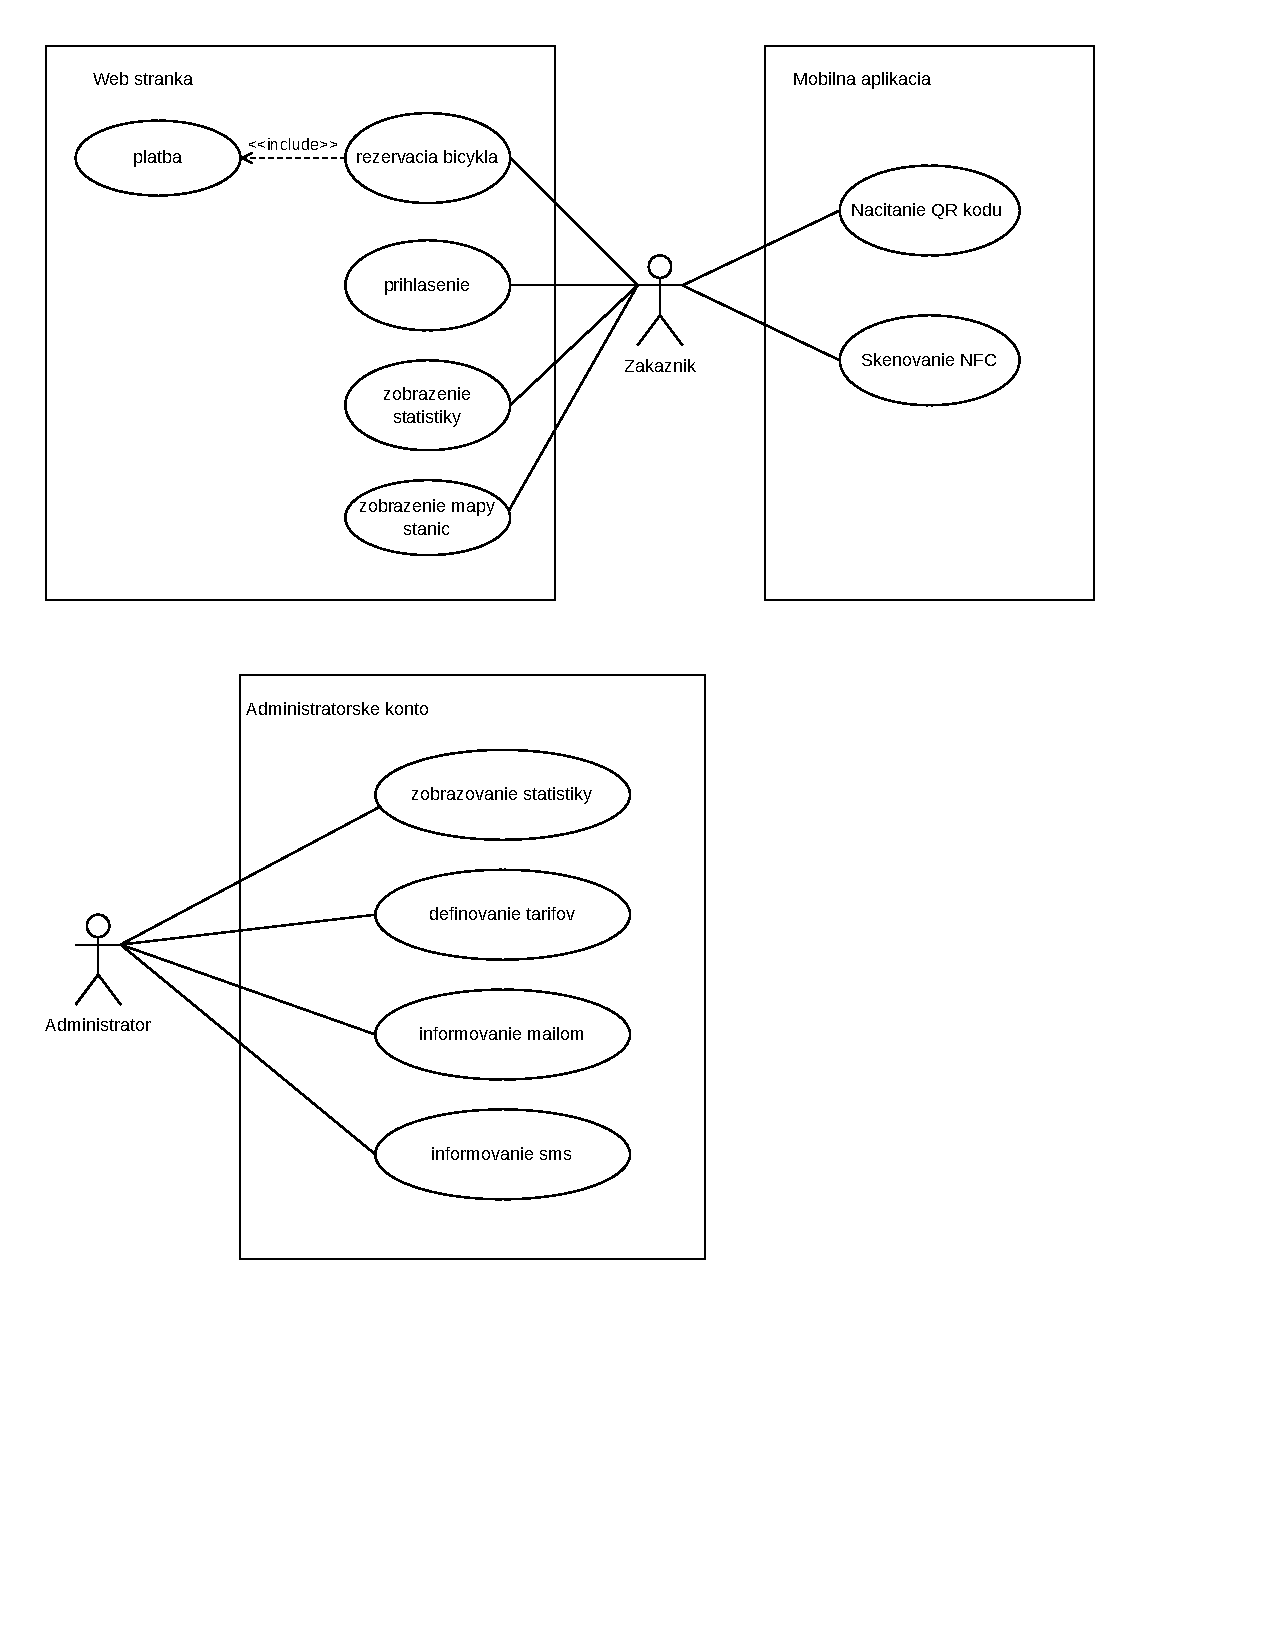
\includepdf[pages=-]{diagrams/pdf/uc.pdf}
\section{Use case tabluľky}
\section{Diagram tried}
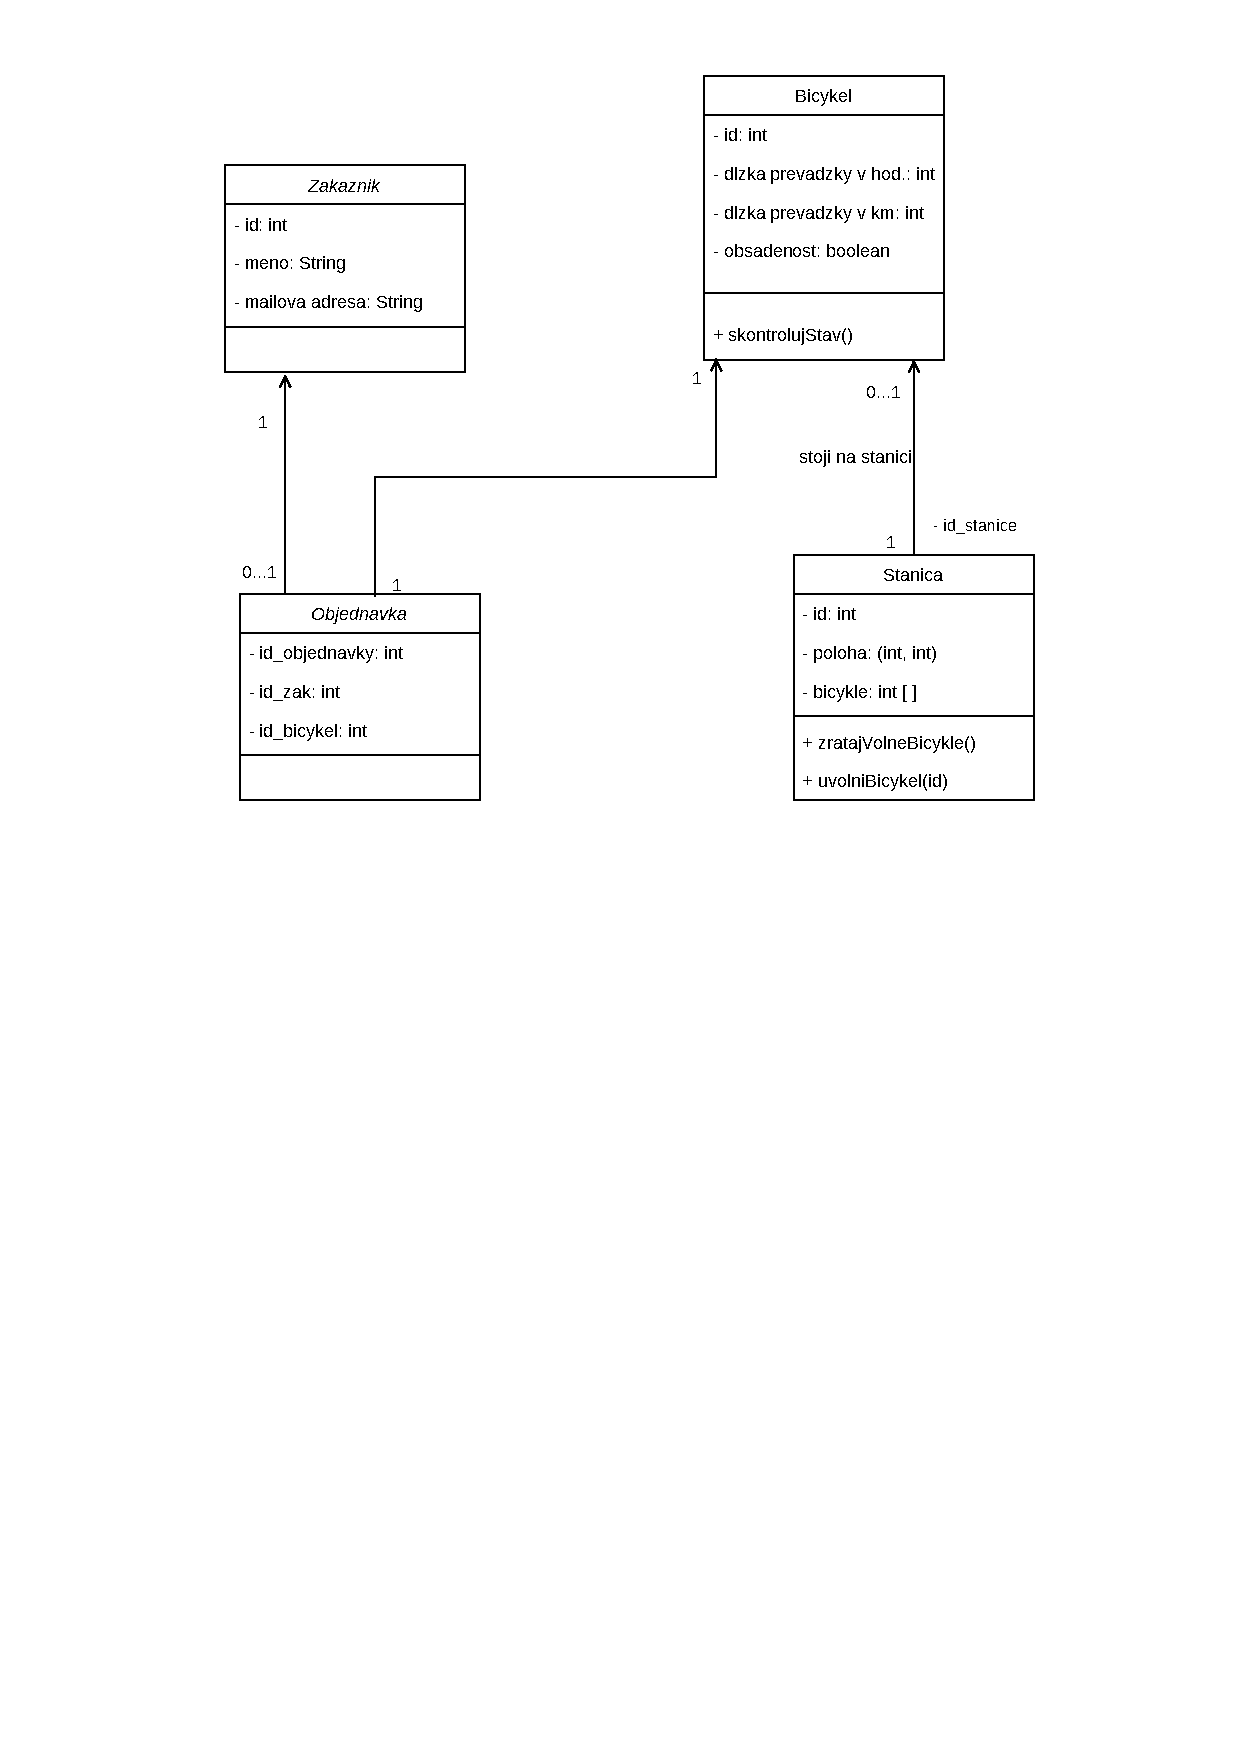
\includepdf[pages=-]{diagrams/pdf/class.pdf}
\end{document}

